\subsection{ANEXO A. Manual de Uso e Instalación}

La herramienta computacional para el análisis de vibración en motores eléctricos
facilita el conocimiento del estado actual de los motores en una planta al mismo
tiempo que permite realizar estudios de evolución históricos y de vibración en
frecuencia, permitiendo de este modo conocer en profundidad que motores podrían
fallar y cual será el elemento, mecánico, que lo hará. Esto permite la realización
de un mantenimiento predictivo, facilitando y mejorando la efectividad y
coordinación de las paradas programadas en una empresa.

Esta herramienta es un sistema Web por lo cual \textbf{NO REQUIERE INSTALACIÓN
EN LA COMPUTADORA}, solo se debe acceder al sitio Web (servidor) el cual se
utilice como \textbf{HOST} para esta.

Para facilitar el acceso al usuario, esta consta de 3 paginas principales,
general, especifica y exhaustiva, además consta de 2 elementos fijos que son el
\textbf{Header}, mostrando la información de la planta y además permitiendo
el regreso a la vista principal (general),  solicitar ayuda y muestra en que
vista se encuentra en el momento. Esto se puede observar en la figura
\ref{img:HeaderHerramienta}.

    \begin{figure}[H]
		\centering
        \caption{Header de la herramienta computacional. }
        
\includegraphics[width=\linewidth]{ManualUsuario/header.png}
        \label{img:HeaderHerramienta}
	\end{figure}

La otra vista constante es la del \textbf{Footer} que ofrece los derechos de autor
y copyright.

    \begin{figure}[H]
		\centering
        \caption{Footer de la herramienta computacional. }
        
\includegraphics[width=\linewidth]{ManualUsuario/footer.png}
        \label{img:FooterHerramienta}
	\end{figure}

El resto de la pantalla se modifica de acuerdo a que pestaña (vista) se observa,
esto es:

\subsubsection{Vista General}
Es la vista principal de la aplicación, esta diseñada para un monitoreo constante
lo que implica que recarga la información cada cierto tiempo (por defecto 30s)
este periodo puede ser modificado únicamente por código y si se desea cambiar debe
comunicarse con el proveedor de servicio.

Esta ventana, se observa en la figura \ref{img:vistaGeneralManual}
cuenta de dos partes fundamentales:

    \begin{figure}[H]
		\centering
        \caption{Vista de la pestaña general de la herramienta computacional. }
        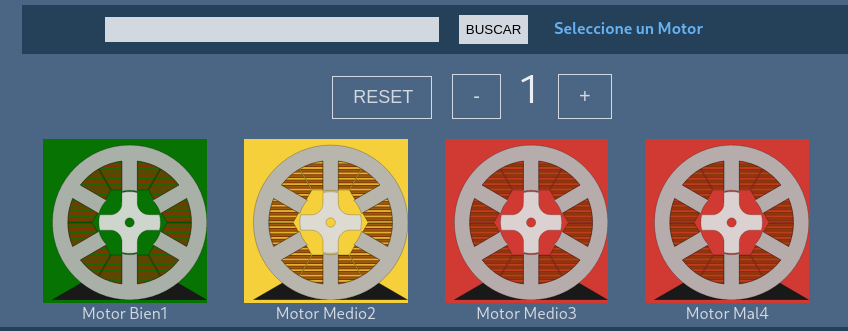
\includegraphics[width=\linewidth]{ManualUsuario/general.png}
        \label{img:vistaGeneralManual}
	\end{figure}

La primera es el despliegue de motores
con un máximo de 12 motores por "pagina" (para modificar esta cantidad comunicarse
con el proveedor de servicios) los cuales indican su código o identificador en
su parte inferior (este código se ingresa al registrar el motor, se recomienda sea
el mismo del de mantenimiento para facilitar su utilización) y un diagrama de
motor con un fondo de color con código correspondiente a su estado, nivel de
vibración y aceleración ajustado a los parámetros solicitados (modificaciones con
el proveedor del servicio); este código es :

\begin{itemize}
    \item  verde: bien.
    \item amarillo: primera alerta.
    \item rojo: segunda alerta.
\end{itemize}

la segunda parte de interés es el buscador y control de paginación, se observa en
la figura \ref{img:buscadoreGeneral}, el buscador permite solicitar la vista
especifica de cualquier motor, buscando por el Identificador del mismo;
el control de paginación permite mostrar otros motores al "pasar" la pagina,
de igual forma permite regresar directamente al principio con el botón de
\textbf{RESET}.

    \begin{figure}[H]
		\centering
        \caption{Controles de paginación en la vista principal. }
        
\includegraphics[width=\linewidth]{ManualUsuario/controles.png}
        \label{img:buscadoreGeneral}
	\end{figure}


\subsubsection{Vista Especifica}
Esta vista permite un nivel de estudio superior ya que es solamente enfocada
a un motor y ofrece la información histórica del mismo, esto lo hace mediante
gráficas y una tabla exportable a Excel.

tiene 3 secciones de trascendencia:

la primera es un encabezado resumen,
se puede apreciar en \ref{img:especificaHeaderManual}; en este se encuentra
el estado del motor como en la vista general, un enlace para solicitar la
vista Exhaustiva y un mensaje con las características del motor o
comentarios adicionales añadidos al momento de la incorporación del motor al
sistema.

    \begin{figure}[H]
		\centering
        \caption{Sección de mensaje en la vista especifica. }
        
\includegraphics[width=\linewidth]{ManualUsuario/especificaMensaje.png}
        \label{img:especificaHeaderManual}
	\end{figure}

La segunda es una serie de gráficas de toda la información histórica, separada
por ejes (x,y,z) y de la aceleración, se muestran después de la palabra
\textbf{Histogramas}, como se observa en la figura \ref{img:especificaGraficasManual}.

    \begin{figure}[H]
		\centering
        \caption{Sección de gráficas en la vista especifica. }
        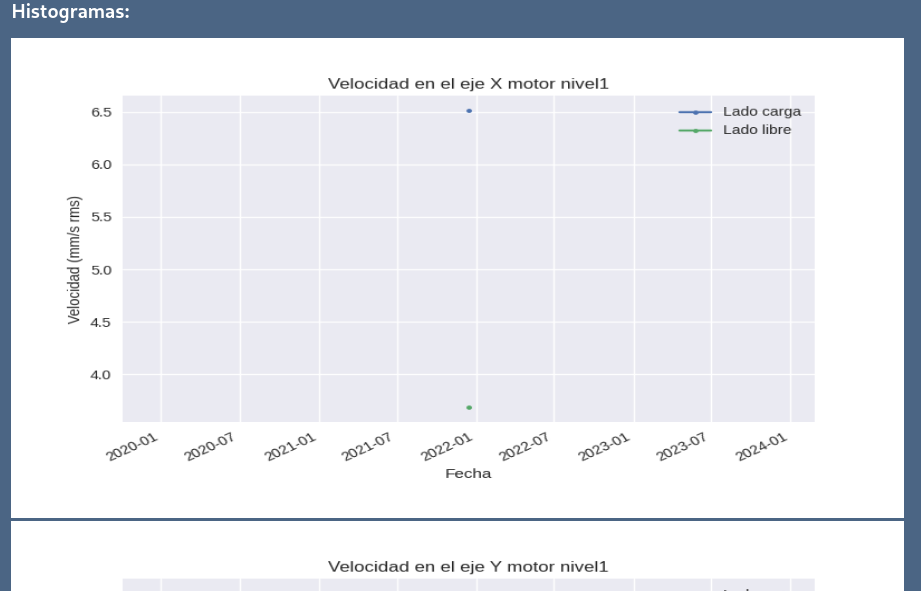
\includegraphics[width=\linewidth]{ManualUsuario/especificaGraficas.png}
        \label{img:especificaGraficasManual}
	\end{figure}

La tercera es una tabla, como se observa en \ref{img:especificaTablaManual}
exportable a Excel, mediante el botón, con toda la información de las mediciones
a lo largo de la historia del sistema, esta posee los campos de:
\begin{itemize}
    \item fecha, en la cual se tomo la medición.
    \item Id Sensor, identificador único, numero de serial, que posee el sensor
        (hardware), asociado.
    \item Lado, ubicación en la cual se tomo la medición, lado libre, lado con
        carga o chumaceras y acoples.
    \item Velocidad vertical, medición de la velocidad, en mm/s, medición rms
    \item Velocidad Horizontal, medición de la velocidad, en mm/s, medición rms
    \item Velocidad Axial, medición de la velocidad, en mm/s, medición rms
    \item Aceleración, medición de la aceleración, en \textbf{g} .
\end{itemize}

\textbf{Nota,} si la tabla no posee todos los campos en su navegador, selecciónela
y utilice las flechas del teclado para redirigirla, o reduzca el tamaño de su
pantalla.

    \begin{figure}[H]
		\centering
        \caption{Sección de la tabla en la vista especifica. }
        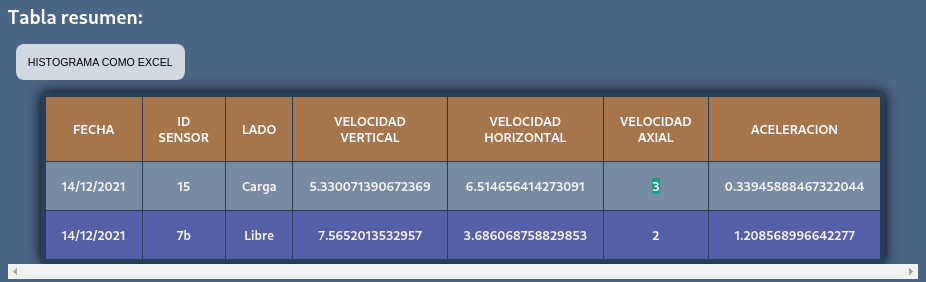
\includegraphics[width=\linewidth]{ManualUsuario/especificaTabla.png}
        \label{img:especificaTablaManual}
	\end{figure}


\subsubsection{Vista Exhaustiva}
Esta vista incluye las mismas características de la vista especifica pero sufre
una modificación en el encabezado resumen, como se puede apreciar en la figura
\ref{img:exhaustivaMensajeManual}
este redirige a la vista principal.

    \begin{figure}[H]
		\centering
        \caption{Sección de mensaje en la vista exhaustiva. }
        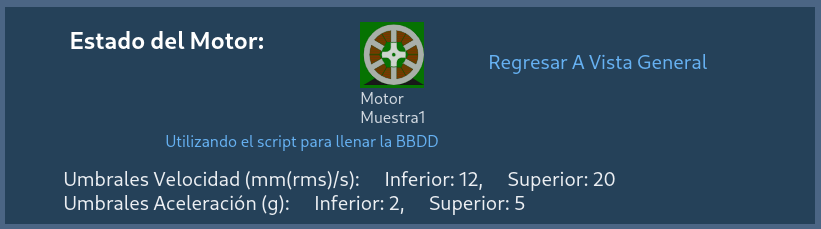
\includegraphics[width=\linewidth]{ManualUsuario/exhaustivaMensaje.png}
        \label{img:exhaustivaMensajeManual}
	\end{figure}



La otra modificación es que se añade otra sección de gráfica en la cual se muestra
la salida de un estudio en frecuencia, permitiendo este su análisis; se observa en
la figura \ref{img:exhaustivaGraficaFourierManual}


    \begin{figure}[H]
		\centering
        \caption{Sección de gráfica de frecuencia en la vista exhaustiva. }
        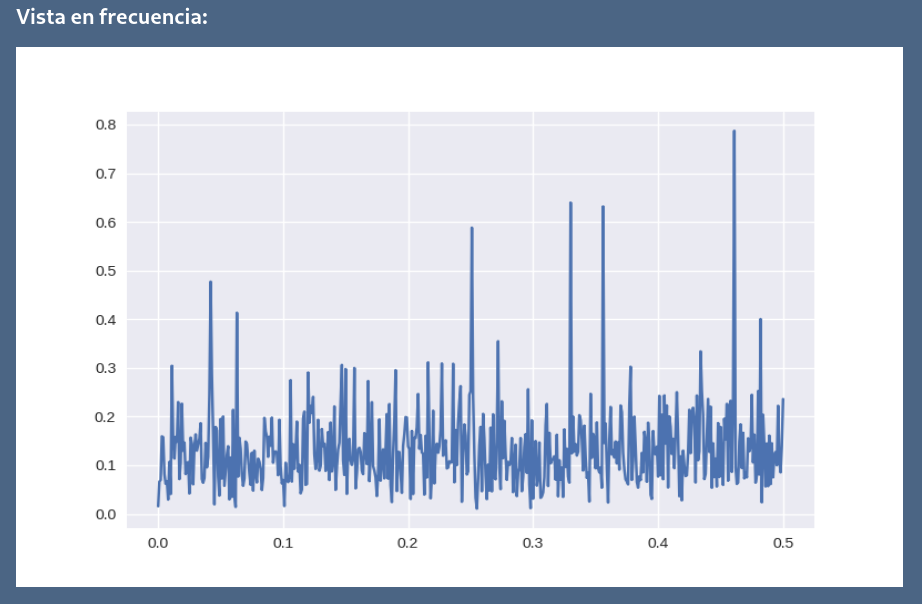
\includegraphics[width=\linewidth]{ManualUsuario/exhaustivaGraficaFourier.png}
        \label{img:exhaustivaGraficaFourierManual}
	\end{figure}




